\subsection{Выбор модели автокодировщика (Попова)}
В качестве данных для проведения вычислительного эксперимента использовались данные WISDM~\cite{wisdm}, представляющие собой набор записей акселерометра мобильного телефона. Каждой записи соответствуют три координаты по осям акселерометра. Набор данных содержит записи движений для 6 классов переменной длины.
При проведении вычислительного эксперимента из каждой записи использовались первые 200 сегментов. Т. к. выборка не сбалансирована, в нее добавлялись повторы записей классов, содержащих количество записей, меньшее чем у большего класса.

Основные эксперименты --- исследование зависимости ошибки классификации от числа параметров и размера выборки --- были проведены как с использованием инструментария на базе библиотеки Theano, так и с использованием инструментария на языке Matlab.
Для оценки качества классификации была проведена процедура скользящего контроля~\cite{cv} при соотношении числа объектов обучающей и контрольной выборки 3:1. Число нейронов на каждом слое задавалось из соотношения 10:6:3. При проведении процедуры скользящего контроля для каждого отсчета количества нейронов было произведено пять запусков. В эксперименте с использованием инструментария на базе Theano при обучении двухслойной нейронной сети проводился мультистарт~\cite{multi}, т.~е. одновременный запуск обучения сети с 8 разными стартовыми значениями параметров для предотвращения возможного застревания алгоритма обучения в локальном минимуме. При оценке качества классификации выбиралась модель с наилучшими результатами. График зависимости ошибки классификации от числа используемых нейронов изображен на рис.~\ref{fig:neurons}.


\begin{figure}[tb!]
 \centering
  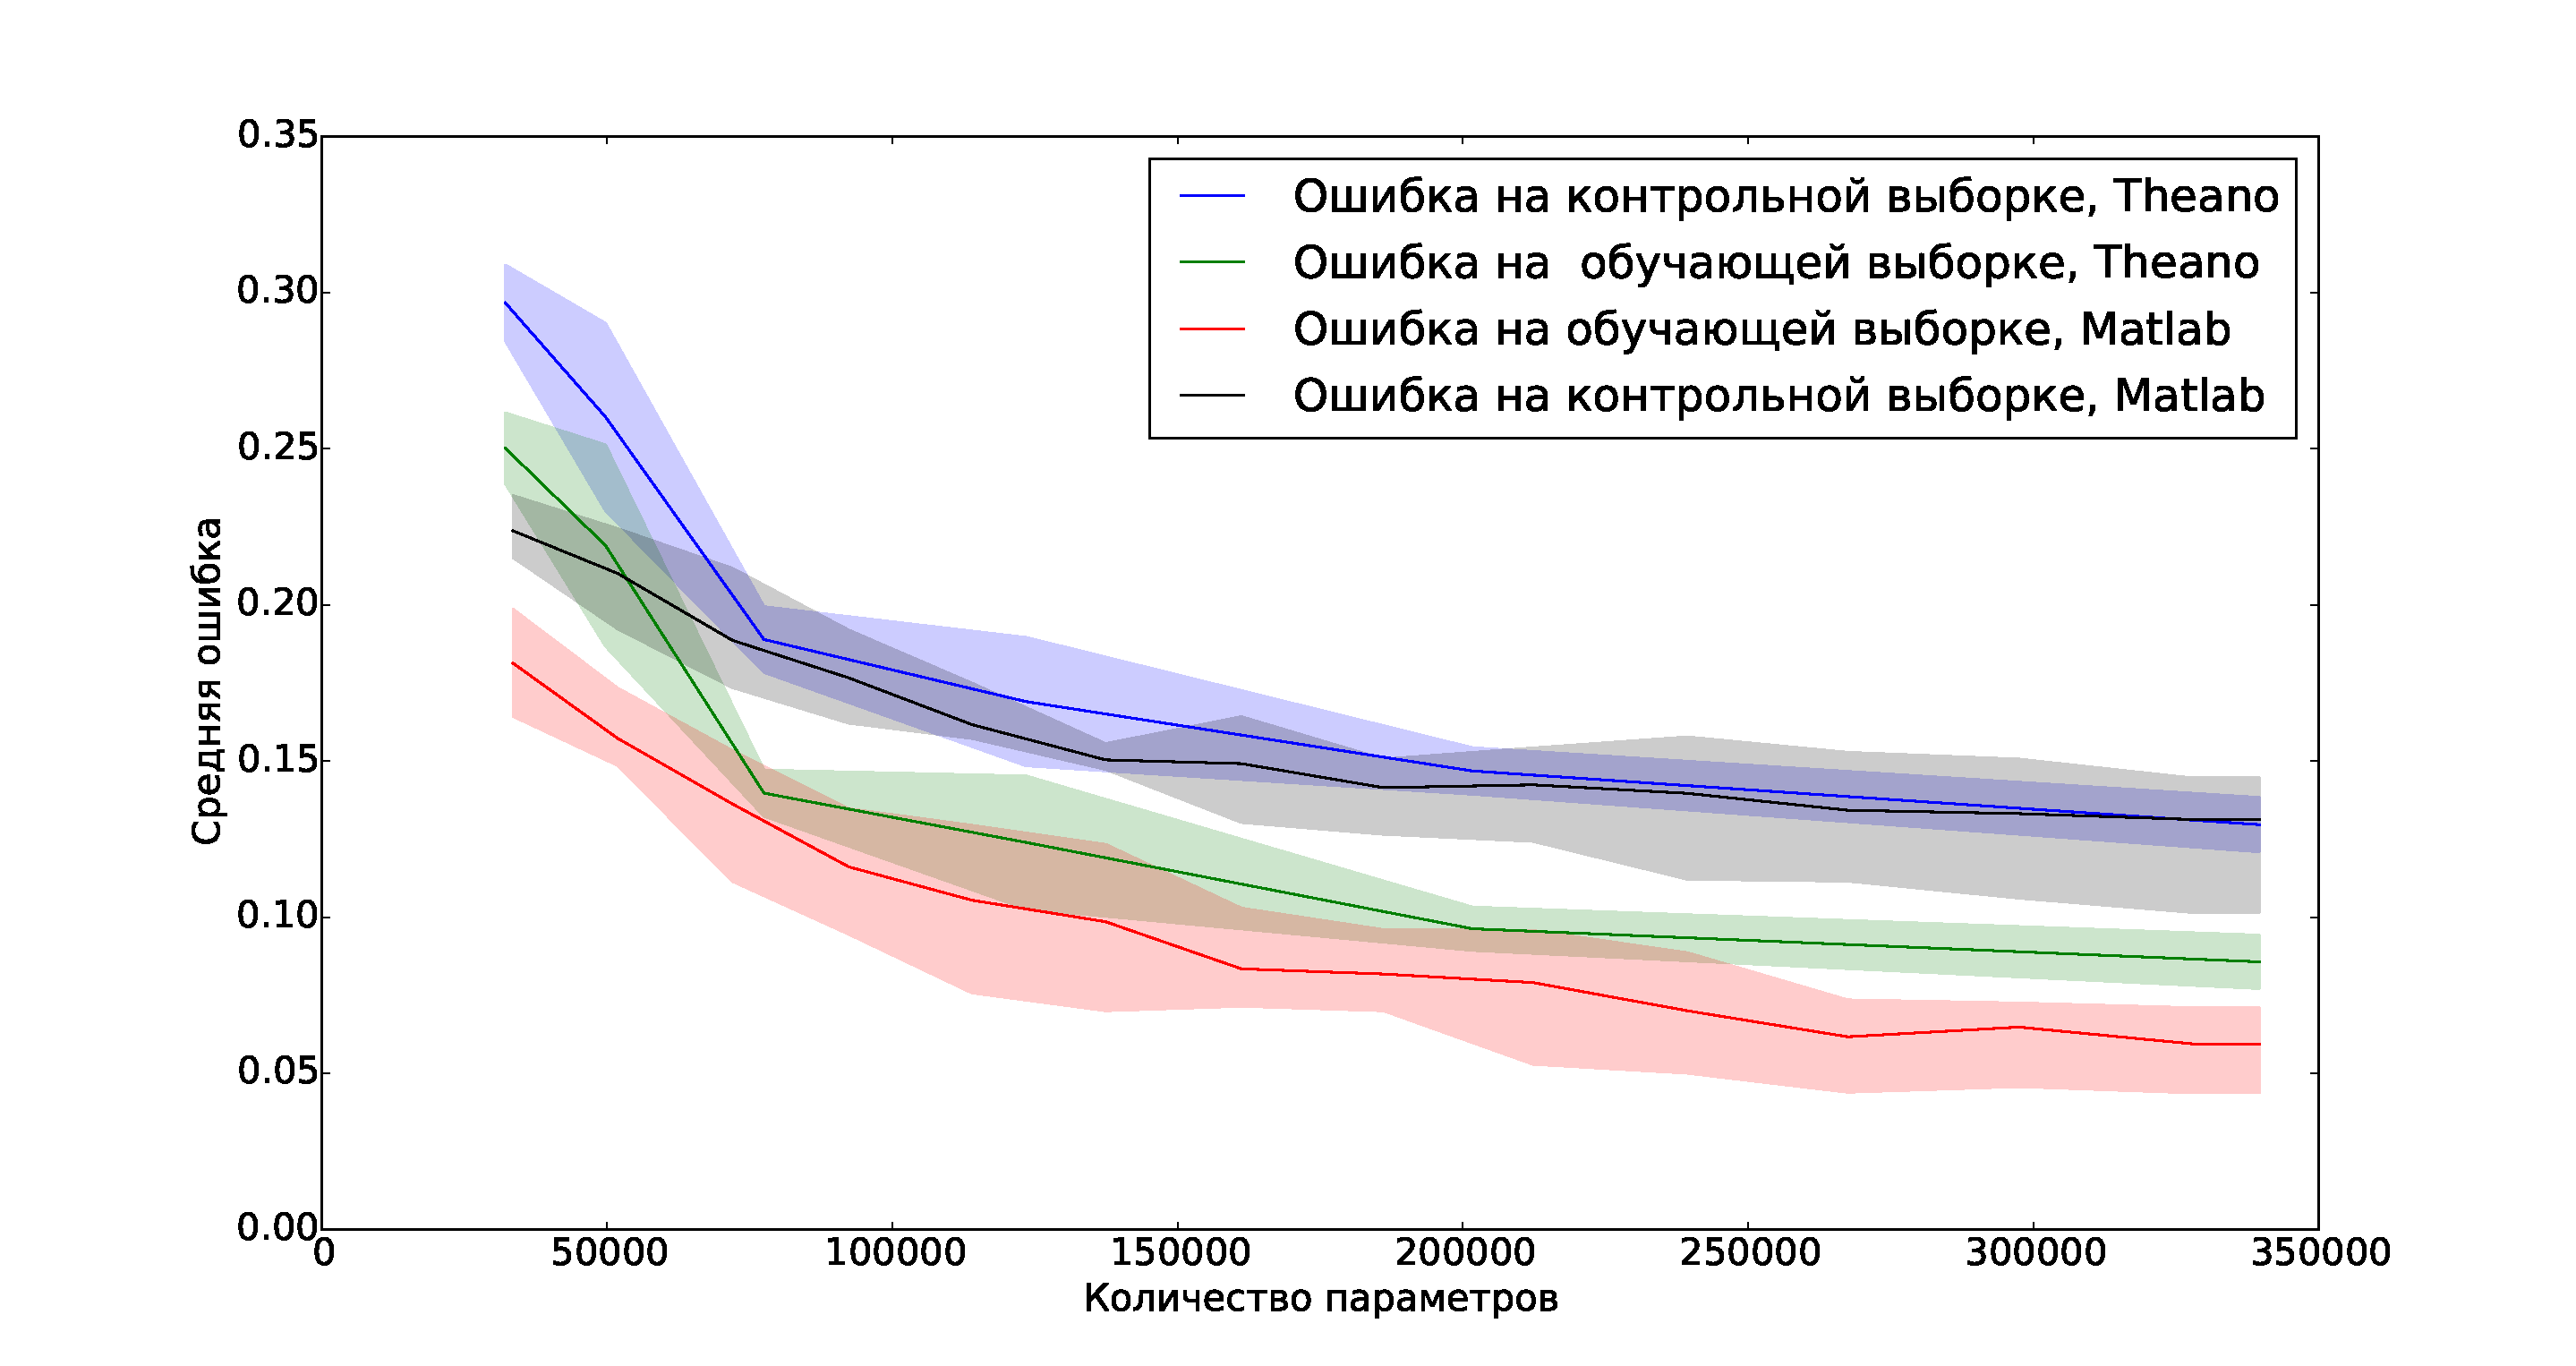
\includegraphics[width=1.0\textwidth]{neurons.pdf}
 \caption{Зависимость ошибки от числа нейронов}
 \label{fig:neurons}
\end{figure}


Для оценки зависимости качества классификации от размера обучающей выборки была проведена кроссвалидация с фиксированным количеством объектов в обучающей выборке (25\% исходной выборки) и переменным размером обучающей выборки. Число нейронов было установлено как 364:224:112. При проведении процедуры скользящего контроля для каждого отсчета было произведено пять запусков. График зависимости ошибки классификации от размера обучающей выборки представлен на рис.~\ref{fig:samples}.


\begin{figure}[tb!]
 \centering
  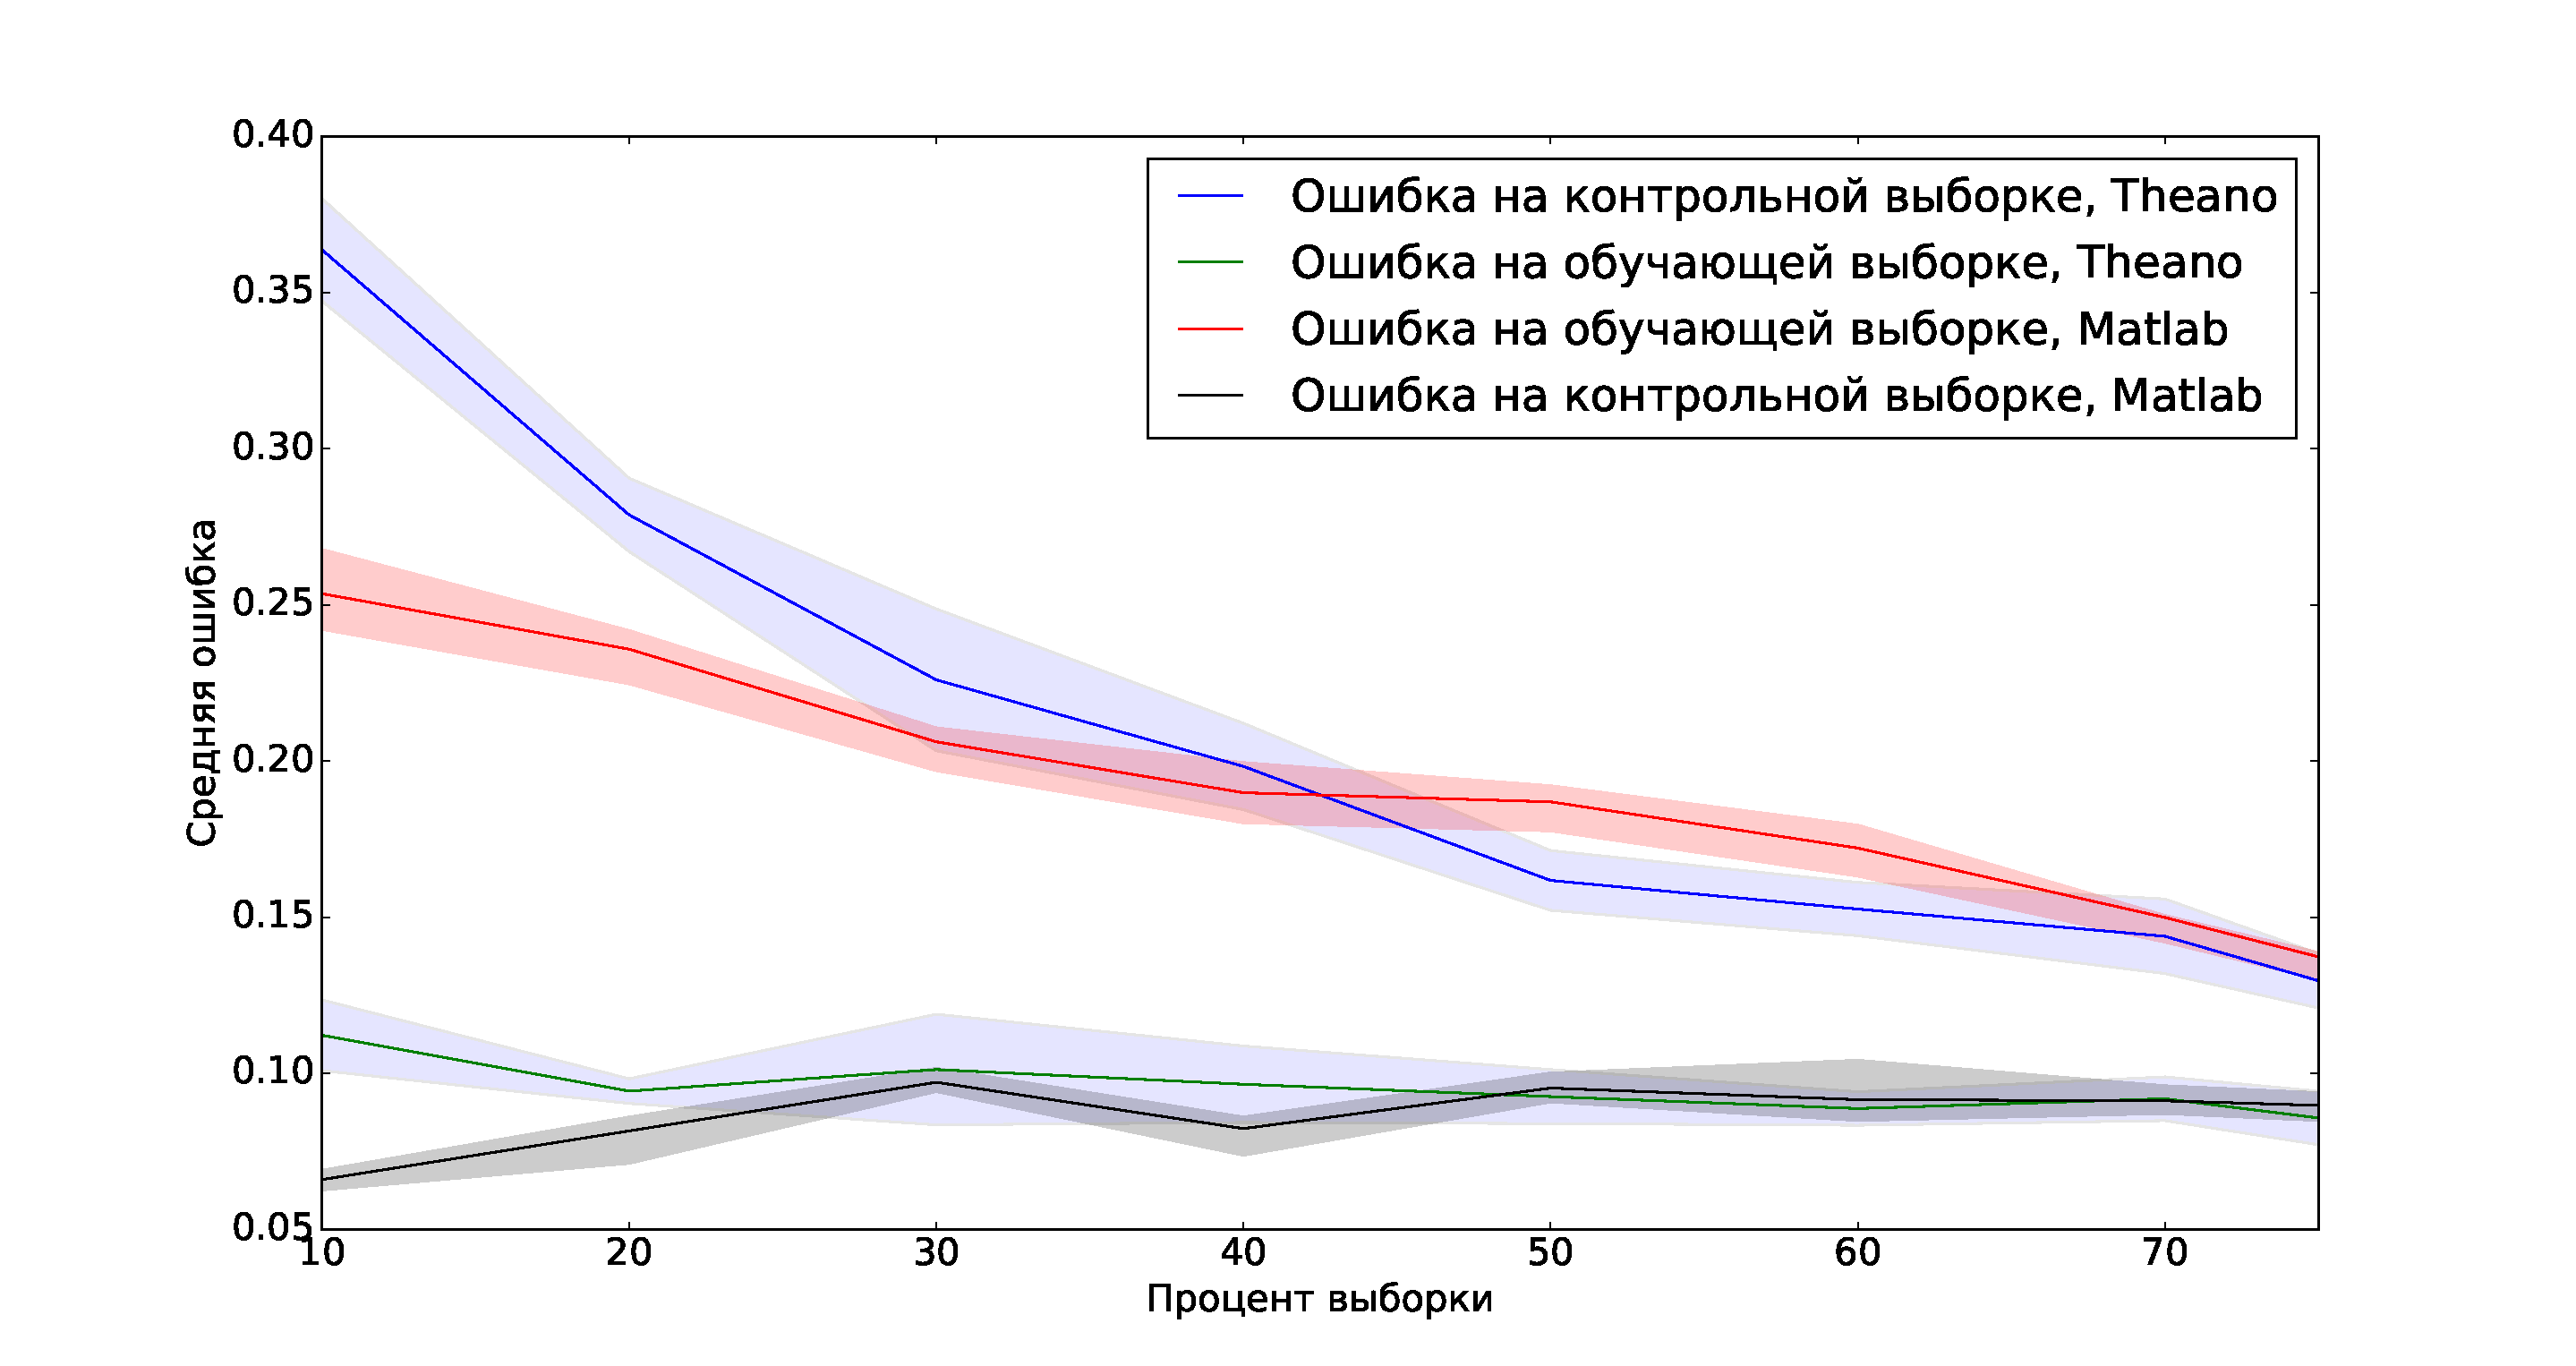
\includegraphics[width=1.0\textwidth]{samples.pdf}
 \caption{Зависимость ошибки от размера обучающей выборки}
 \label{fig:samples}
\end{figure}


Для исследования скорости работы процесса обучения нейросети в зависимости от конфигурации Theano был сделан следующий эксперимент:
проводилось обучение двухслойной нейросети на основе подсчитанных заранее параметров ограниченной машины Больцмана~\eqref{eq:rbm} и автокодировщика~\eqref{eq:ae}. Обучение проходило за 100 итераций. При обучении алгоритм запускался параллельно с $n$ разными стартовыми позициями, $n \in \{1,\dots,4\}.$ Число нейронов было установлено как 300:200:100.
Запуск осуществлялся со следующими конфигурациями Theano:
\begin{itemize}
\item вычисление на центральном процессоре, задействовано
одно ядро;
\item вычисление на центральном процессоре, задействовано четыре ядра;
\item вычисление на центральном процессоре, задействовано восемь ядер;
\item вычисление на графическом процессоре.
\end{itemize}

Результаты эксперимента приведены на рис.~\ref{fig:speed}. Как видно из графика, вычисление с использованием CUDA показывает значительное ускорение по сравнению с вычислением на центральном процессоре.

\begin{figure}[tb!]
 \centering
  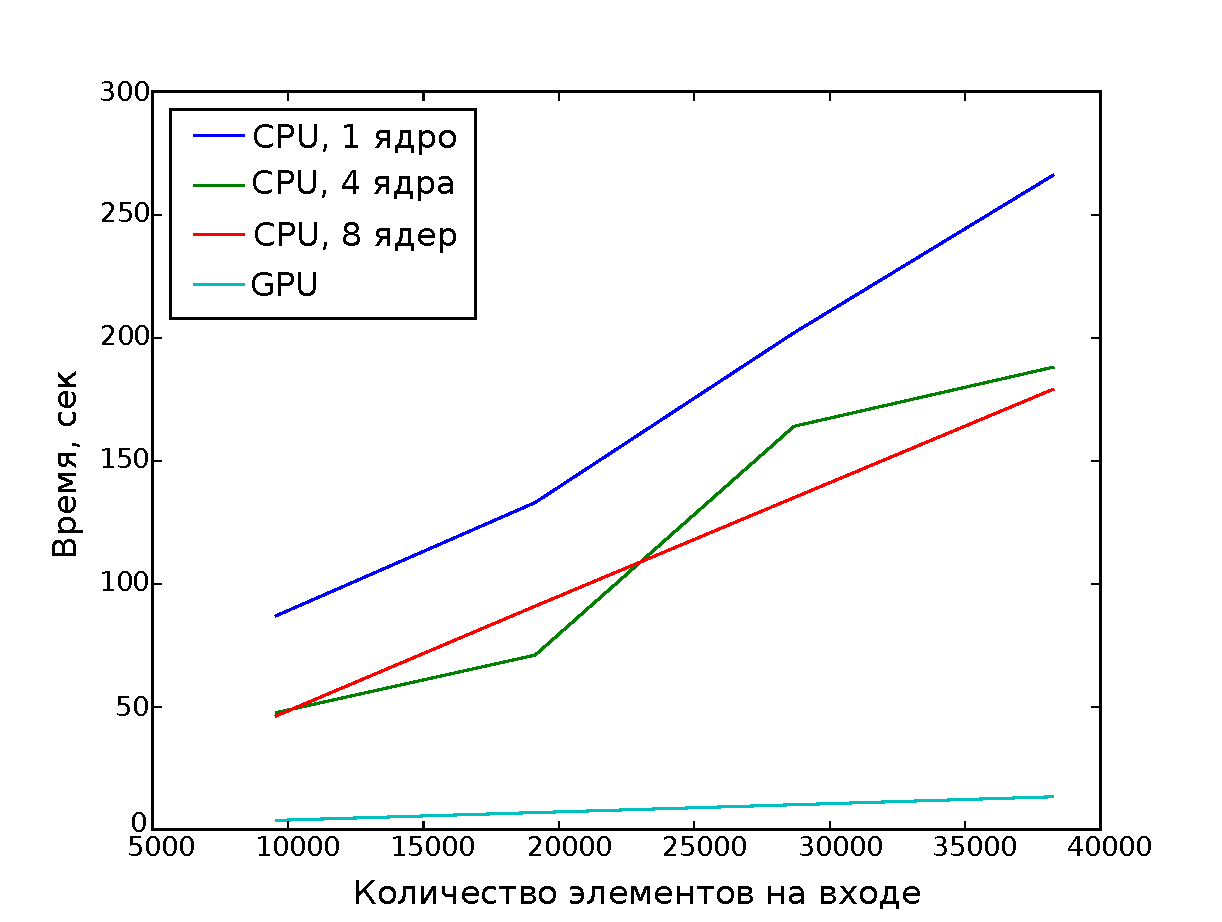
\includegraphics[width=0.8\textwidth]{result.pdf}
 \caption{Результаты эксперимента по исследованию скорости процесса обучения}
 \label{fig:speed}
\end{figure}



\subsection{Evidence (АиТ)}
Для анализа свойств предложенного критерия субоптимальности в задачах регрессии и классификации, а также методов получения нижних оценок правдоподобия модели в задачах выбора моделей был проведен ряд вычислительных экспериментов на выборках Boston Housing, Protein Structure, а также на небольшой подвыборке YearPredictionMSD (далее --- Boston, Protein и MSD)~\cite{UCI} {и подвыборке изображений рукописных цифр MNIST~\cite{mnist}}.

{Для выборок Boston, Protein и MSD} была рассмотрена задача регрессии
\[
	\mathbf{y} = \mathbf{f}(\mathbf{X}, \mathbf{w}) + \boldsymbol{\varepsilon}, \quad  \boldsymbol{\varepsilon} \sim \mathcal{N}(\mathbf{0}, \mathbf{I}), \quad \mathbf{f} \in \mathfrak{F}.
\]

В качестве множества моделей $\mathfrak{F}$ были рассмотрены  нейросети с одним скрытым слоем и softplus-функцией активации:
\begin{equation}
\label{eq:model}
	\mathbf{f}(\mathbf{w}, \mathbf{X}) =   \textbf{softplus}\bigl(\mathbf{X} \mathbf{W}_1 \bigr)  \mathbf{W}_2,
\end{equation}
где $\mathbf{W}_1 \in \mathbb{R}^{n\times n_1}$ --- матрица параметров скрытого слоя нейросети, $\mathbf{W}_2 \in \mathbb{R}^{n_1\times 1}$ --- матрица параметров выходного слоя нейросети, {$\textbf{softplus}(\mathbf{X}) = \textbf{log}\bigl(1+\textbf{exp}(\mathbf{X})\bigr)$}.

{Для выборки Boston также было рассмотрено множество моделей с тремя скрытыми слоями, построенных аналогично однослойной модели~\eqref{eq:model}. Размер каждого слоя равнялся 50.}

{Для выборки MNIST была рассмотрена задача бинарной классификации: из выборки были взяты только объекты, соответствующие цифрам 7 и 9. Размерность выборки была понижена с 784 до 50 методом главных компонент аналогично~\cite{firefly}. Для анализа моделей, полученных в случае высокой вероятности переобучения, из обучающей выборки были взяты первые 500 объектов. В качестве модели рассматривалась нейросеть с тремя скрытыми слоями}
\[
    \mathbf{f}(\mathbf{w}, \mathbf{X}) =   \boldsymbol{\sigma}(\textbf{softplus}\bigl(  \textbf{softplus} \bigl(\textbf{softplus}\bigl(\mathbf{X} \mathbf{W}_1 \bigr)  \mathbf{W}_2 \bigr) \mathbf{W}_3 \bigr) \mathbf{W}_4),
\]
{где $\boldsymbol{\sigma}(\mathbf{X}) = \bigl(1+\textbf{exp}(\mathbf{-X})\bigr)^{-1}$  --- сигмоида, $\mathbf{W}_1, \dots, \mathbf{W}_4$ --- параметры нейросети.}



Во всех экспериментах исходная выборка $\mathfrak{D}$ разбивалась на обучающую и контрольную подвыборки:
$
	\mathfrak{D} = \mathfrak{D}_\textnormal{train} \sqcup \mathfrak{D}_\textnormal{text}.
$

Оптимизация параметров производилась на подвыборке $\mathfrak{D}_\textnormal{train}$. Для контроля переобучения некоторых алгоритмов из обучающей выборки $\mathfrak{D}_\textnormal{train}$ формировалась валидационная выборка $\mathfrak{D}_\textnormal{valid}$, на которой не проводилась оптимизация параметров  модели. Мощность валидационной выборки $\mathfrak{D}_\textnormal{valid}$ составляла 0,1 мощности обучающей выборки  $\mathfrak{D}_\textnormal{train}$, объекты для валидационной выборки выбирались случайным образом независимо для каждого старта алгоритма.
Качество полученных моделей проверялось на подвыборке $\mathfrak{D}_\textnormal{test}.$ Критерием качества модели выступали среднеквадратичное отклонение вектора $\mathbf{y}$ от вектора $\mathbf{f}(\mathbf{w}, \mathbf{X})$ (RMSE) {в случае задачи регрессии и доля верно предсказанных меток класса (Accuracy) в задаче классификации}, а также { соответствующие критерии } при возмущении элементов выборки:
\begin{equation}
\label{eq:rmse}
	\textnormal{RMSE}_{\sigma} =\textnormal{RMSE}\bigl(\mathbf{f}( \mathbf{w}, \mathbf{X}+\boldsymbol{\varepsilon}), \mathbf{y}\bigr),  \quad \boldsymbol{\varepsilon} \sim \mathcal{N}(\mathbf{0}, \sigma \mathbf{I}).
\end{equation}

Были рассмотрены шесть алгоритмов.
\begin{enumerate}%[label={\arabic{enumi}.\arabic*}] 
\item Базовый алгоритм: оптимизация параметров без валидации и ранней остановки. Оптимизация проводилась с использованием стохастического градиентного спуска~\eqref{eq:sgd}. Для данного алгоритма априорное распределение $p(\mathbf{w}|\mathbf{f})$ не использовалось.
\item Алгоритм с валидацией. Для контроля переобучения во время оптимизации качество модели оценивалось на валидационной выборке $\mathfrak{D}_\textnormal{valid}$. Для данного алгоритма априорное распределение также не использовалось.
\item Алгоритм с валидацией и введенным априорным распределением. В качестве априорного распределения рассматривается распределение вида
$
	\mathbf{w} \sim \mathcal{N}(\mathbf{0}, \alpha \mathbf{I}), 
$
где $\alpha$ --- дисперсия.

\item Нахождение вариационной нижней оценки с использованием стохастического градиентного спуска.
\item Нахождение вариационной нижней оценки с использованием стохастической динамики Ланжевена.
\item Нахождение вариационной нижней оценки с аппроксимацией нормальным распределением ~\eqref{eq:gaus}.
\end{enumerate}




Параметры модели выбирались из точек мультистарта (алгоритмы 1---5) или порождались из распределения $\hat{q}$ (алгоритм 6). Количество точек мультистарта: $r=10$ {для задач регрессии и $r=25$ для задачи классификации}.
Для алгоритмов 2---6 применялась ранняя остановка: каждые $\tau_\textnormal{val}$ итераций производилась оценка внутреннего критерия качества модели. В качестве критерия остановки применялось следующее условие: значение внутреннего критерия качества не улучшалось $3\tau_\textnormal{val}$ итераций. Для разных алгоритмов внутренним критерием качества выступали различные величины:
\begin{enumerate}
\item функция потерь $L$~\eqref{eq:loss_func} на валидационной выборке $\mathfrak{D}_\textnormal{valid}$ для алгоритмов $2,3$,
\item вариационная нижняя оценка правдоподобия~\eqref{eq:elbo} на обучающей выборке $\mathfrak{D}_\textnormal{train}$ для алгоритмов $4,5,6$.
\end{enumerate}

Для каждой модели назначались различные значения параметра $\alpha (\alpha \in \{10, \dots, 10^9\})$ и длины шага оптимизации $\gamma$, отбирались наилучшие модели. %Пример матрицы качества модели в зависимости от гиперпараметров приведена на рис.~\ref{fig:hypermatrix}.



Описание эксперимента представлено в табл.~1. Результаты экспериментов представлены в табл.~2. На рис.~\ref{fig:noise_in_data} представлен график зависимости $\textnormal{RMSE}_{\sigma}$ от параметра~$\sigma$~{ для однослойных моделей}. 

\begin{table}[!htbp]
\captionsetup{justification=raggedright,singlelinecheck=false}
\label{table1}
\caption*{\textbf{Таблица 1. Описание выборок для экспериментов}}
\footnotesize
\centering

\begin{tabular}{ | p{2cm} |p{2cm} | p{2cm} | p{2cm} | p{2cm} | p{2cm} | }
\hline
Выборка $\mathfrak{D}$ & Интервал валидации, $\tau_\textnormal{val}$ & Количество объектов, $m$ & Количество признаков, $n$ & Размер подвыборки, $\hat{m}$ &  Размер скрытого слоя, $n_1$ \\
\hline
Boston Housing & 100 & 506 & 13 & $\hat{m} = m$ & 50 \\
\hline
Protein & 1000 & 45000 & 9 & $\hat{m} = 200$ & 100 \\
\hline
MSD & 1000& 5000 & 91 & $\hat{m} = 50$ & 100\\
\hline
MNIST & 100  & 500 & 50 & $\hat{m} = 100$ & 50\\ 
\hline
\end{tabular}
\end{table}


\newcommand{\specialcell}[2][c]{%
  \begin{tabular}[#1]{@{}c@{}}#2\end{tabular}}

\begin{table}[htbp!]
\captionsetup{justification=raggedright,singlelinecheck=false}
\centering
\label{table2}
\caption*{\textbf{Таблица 2. Результаты эксперимента}}
\footnotesize
\begin{tabular}{ | c | c | c | c | c | c | c |}

\hline
&\multicolumn{6}{|c|}{Алгоритмы}  \\
\hline
Выборка $\mathfrak{D}$ & 1 & 2 & 3 & 4 & 5 & 6 \\
\hline
\multicolumn{7}{|c|}{Результаты, RMSE/Accuracy}  \\

\hline
\specialcell{ Boston,  \\один  слой} & 8,1  $\pm$ 2,0 & 5,9 $\pm$ 0,7 & 5,2 $\pm$ 0,6 & $\mathbf{3,7 \pm 0,2}$ & 6,7 $\pm$ 0,7 & 5,0 $\pm$ 0,4 \\
\hline
Boston, 3 слоя & 7,1 $\pm$ 1,3 & 4,3 $\pm$ 0,1 & 4,4 $\pm$ 0,4 & $\mathbf{3,2 \pm 0,06}$ & 4,6 $\pm$ 0,4 & 6,8 $\pm$ 1,6 \\
\hline
Protein & 5,1 $\pm$ 0,0 & 5,1 $\pm$ 0,0 & 5,1 $\pm$ 0,0 & 5,1 $\pm$ 0,0 & 5,1 $\pm$ 0,0 & $\mathbf{5,0 \pm 0,1}$ \\
\hline
MSD & 12,2 $\pm$ 0,0 & $\mathbf{10,9 \pm 0,1}$ & $\mathbf{10,9 \pm 0,1}$ & 12,2 $\pm$ 0,0 & 12,9 $\pm$ 0,0 & 19,6 $\pm$ 3,6  \\
\hline
MNIST & 0,985 $\pm$ 0,002 & 0,984 $\pm$ 0,002 & $\mathbf{0,986 \pm 0,002}$ & 0,914 $\pm$ 0,005 & 0,979 $\pm$ 0,003 & 0,971 $\pm$ 0,001 \\
\hline

\multicolumn{7}{|c|}{Результаты, $\textnormal{RMSE/Accuracy}_{0,5}$}  \\
\hline
\specialcell{ Boston,  \\один  слой} & 43,9  $\pm$ 9,4 & 18,6 $\pm$ 2,0 &  15,8 $\pm$ 2,3 & $\mathbf{11,9 \pm 1,1}$ & 20,3 $\pm$ 3,1 & 18,2 $\pm$ 3,3 \\
\hline
Boston, 3 слоя & 23,4 $\pm$ 4,9 & 18,7 $\pm$ 2,8 & 18,3 $\pm$ 3,0 & \bf 9,0 $\pm$ 0,7 & 14,5 $\pm$ 2,6 &  15,2 $\pm$ 2,7 \\
\hline
Protein & 19,5 $\pm$ 0,3 & 18,5 $\pm$ 0,5 & 18,6 $\pm$ 0,3 & $\mathbf{16,7 \pm 0,3}$ & 19,3 $\pm$ 0,6 & 19,7 $\pm$ 3,7  \\
\hline
MSD & 178,3 $\pm$ 0,8 & $\mathbf{121,3 \pm 4,5}$ & 123,7 $\pm$ 2,5 & 175,8 $\pm$ 1,0 & 203,8 $\pm$ 1,4 & 292,0 $\pm$ 2,0 \\
\hline
MNIST & 0,931 $\pm$ 0,004 & 0,929 $\pm$ 0,006 & $\mathbf{0,934 \pm 0,007}$ & 0,857 $\pm$ 0,007 & 0,919 $\pm$ 0,008 & 0,916 $\pm$ 0,004 \\
\hline


\multicolumn{7}{|c|}{Результаты, $\textnormal{RMSE/Accuracy}_{1,0}$}  \\
\hline
\specialcell{ Boston,  \\один  слой} & 120,9 $\pm$ 33,4 & 42,5 $\pm$ 6,3 & 32,5 $\pm$ 6,0 & $\mathbf{25,7 \pm 3,2}$ & 42,4 $\pm$ 5,7 & 41,3 $\pm$ 6,3  \\
\hline
Boston, 3 слоя & 46,1 $\pm$ 15,8 & 40,5 $\pm$ 5,3 & 38,6 $\pm$ 8,0 & \bf 16,5 $\pm$ 2,5 & 30,4 $\pm$ 7,9 & 26,2 $\pm$ 6,9 \\
\hline
Protein & 37,0 $\pm$ 0,8 & 34,4 $\pm$ 1,1 & 35,0 $\pm$ 1,0 & $\mathbf{30,6 \pm 0,6}$ & 36,6 $\pm$ 1,1 & 35,0 $\pm$ 8,1 \\
\hline
MSD & 319,6 $\pm$ 1,4 & $\mathbf{217,5 \pm 8,2}$ & 221,9 $\pm$ 4,2 & 314,8 $\pm$ 1,8 & 363,7 $\pm$ 1,9 & 521,6 $\pm$ 3,1  \\
\hline
MNIST & $\mathbf{0,814 \pm 0,010 }$& 0,808 $\pm$ 0,010 &  0,812 $\pm$ 0,008 & 0,772 $\pm$ 0,010 & 0,802 $\pm$ 0,009 & 0,800 $\pm$ 0,009 \\
\hline


\multicolumn{7}{|c|}{Сходимость алгоритмов, тыс. итераций  }  \\
%Выборка $\mathbf{X}$ & Алгоритм 1 & Алгоритм 2 & Алгоритм 3 & Алгоритм 4 & Алгоритм 5 & Алгоритм 6 \\
\hline
\specialcell{ Boston,  \\один  слой} &  25 & 25 & 25 & 14 & 10 & 27 \\
\hline
Boston, 3 слоя &  25 & 4 & 9 & 10 & 1 & 6 \\
\hline
Protein &   60 & 40 & 80 & 40 & 75 & 85 \\
\hline
MSD &  250 & 330 & 335 &  250 & 460 & 120  \\
\hline
MNIST &  1 & 6 & 3 &  13 & 3 & 25  \\
\hline
\end{tabular}
\end{table}





Модели имеют достаточно большое число параметров, поэтому в ходе оптимизации параметров может произойти переобучение. На выборке Boston Housing базовый алгоритм (1) показал наихудший результат в силу переобучения, при этом алгоритм 4 показал лучший результат по сравнению с алгоритмами 2 и 3. 
В данном случае использование вариационной оценки предпочтительнее алгоритмов, основанных на кросс-валидации. На выборке Protein все алгоритмы показали схожие результаты. На выборке MSD алгоритмы 4,5,6 показали худший результат в сравнении с алгоритмами, использующими валидационную подвыборку. Наихудший результат показал алгоритм 6, что говорит о значительном отличии апостериорного распределения параметров~\eqref{eq:posterior} от нормального.  

Алгоритм 6 показал низкое качество~\eqref{eq:rmse} при возмущении объектов выборки {в большинстве экспериментов}. В {трех} экспериментах наилучшие показатели по данному критерию показал алгоритм 4. Заметим, что алгоритм 5, являющийся модификацией алгоритма 4, показал худшие результаты как по RMSE, так и по RMSE при возмущении объектов выборки. 
{На выборке MNIST алгоритм 4 показал результаты значительно хуже остальных алгоритмов. В целом результаты по данному алгоритму схожи с результатами, описанными в~\cite{early}: в отличие от алгоритма 5 алгоритм 4, основанный на стохастическом градиентном спуске, дает заниженную оценку правдоподобия при приближении параметров к точке экстремума. } Алгоритм 5, основанный на динамике Ланжевена, также показал худшее время сходимости~{на выборках MSD и Protein}. Возможным дальнейшим улучшением качества этого алгоритма является введение дополнительной корректирующей матрицы, обеспечивающей лучшее время схождения параметров к апостериорному распределению параметров~\cite{langevin}.

Программное обеспечение для проведения экспериментов и проверки результатов  находится в~\cite{my_src}. 





\subsection{Оптимизация гиперпараметров}
Для анализа рассматриваемых алгоритомв оптимизации гиперпараметров был проведен ряд вычислительных экспериментов на выборках MNIST~\cite{mnist}, WISDM~\cite{wisdm}, а также на синтетических данных.

Рассматривались следующие критерии качества:
\begin{enumerate}
\item Наилучшее значение $\hat{Q} = \max_{j \in \{1, \dots, l\}}Q^j$.
\item Среднее число итераций алгоритма для сходимости. Под данным показателем понимается число шагов оптимизациии гиперпараметров, при котором ошибка $Q$ изменяется не более чем на 1\% от своего наилучшего значения:
\[
    \argmin_{j}: \frac{Q^j - Q^0}{\hat{Q} - Q^0} \geq 0.99,
\]
где $Q^0$ --- значение функции $Q$ до начала оптимизации гиперпараметров.

\item Внешний критерий качества моделей $E$:
\[
    E = \text{RMSE} = \left (\frac{1}{m}\sum_{1}^m (f(\mathbf{x}_i, \mathbf{w})-y_i)\right)^{\frac{1}{2}}
\]
в случае задачи регрессии,
\[
    E = \text{Accuracy} = 1 - \frac{1}{m}\sum_1^m [f(\mathbf{x}_i, \mathbf{w}) \neq y_i]
\]
в случае задачи классификации.

\item Внешний критерий качества моделей $E_\sigma$ при возмущении параметров модели:
\[
    E_\sigma = \text{RMSE}_\sigma = \left (\frac{1}{m}\sum_{1}^m (f(\mathbf{x}_i, \mathbf{w} + \boldsymbol{\varepsilon}-y_i)\right)^{\frac{1}{2}}, \quad \boldsymbol{\varepsilon} \sim \mathcal{N}\bigl(\mathbf{0}, \sigma\mathbf{I}\bigr).
\]
\end{enumerate}

%Для каждого алгоритма для синтетической выборки было проведено 50 повторений, результаты были усреднены. 
%Для остальных выборок было проведено 5 повторений. 
В качестве улучшаемого алгоритма рассматривался случайный поиск параметров с количеством итераций поиска, совпадающих с количеством итераций оптимизации гиперпараметров $l$: $l=50$ для синтетической выборки и выборки WISDM, $l=25$ для выборки MNIST. Рассмаитрваемые алгоритмы представлены в Табл.~\ref{table:algo_descr}. Пример поведения траекторий параметров под действием алгоритмов приведен на Рис.~\ref{fig:traj}. В качестве функций $Q$ и $L$ рассматривались функции кросс-валидации~\eqref{eq:cv} с $k=4$ и вариацонной оценки правдоподобия~\eqref{eq:elbo}. 

\begin{table}
\small
% Алгоритм & Тип алгоритм & Время & Плюсы & Минусы 

\begin{tabularx}{\textwidth}{|X|X|X|X|}
\hline
\bf Алгоритм & \bf Тип алгоритма & \bf Сложность работы одной итерации & \bf Предположения для корректности  \\ 
Случайный поиск & стохастический & $O(\eta s |\hat{\mathfrak{D}}|)$& -  \\ \hline
Жадный алгоритм~\cite{hyper_greed} & градиентный & $O(\eta (s+h) |\hat{\mathfrak{D}}|)$ & $\mathbf{H}(\boldsymbol{\theta}) = \mathbf{I}$  \\ \hline
HOAG~\cite{hyper_hoag} & градиентный & $O(\eta s |\hat{\mathfrak{D}}| + h^2 |\hat{\mathfrak{D}}| + \text{o}),$ где $o$ --- время решения уравнения пункте 3&  первые производные $Q$ и вторые производные $L$ --- липшецевы;  $\text{det}\mathbf{H} \neq \mathbf{0}$;  \\ \hline
DrMAD~\cite{hyper_mad} & градиентный &$O(\eta s |\hat{\mathfrak{D}}|)$ & Траектория оптимизации параметров $\boldsymbol{\theta}$ = $\boldsymbol{\theta}_0, \dots \boldsymbol{\theta}_\eta$ --- линейная \\ \hline
\end{tabularx}

\caption{Основные свойства рассматриваемых алгоритмов}
\label{table:algo_descr}

\end{table}


\begin{figure}

    \begin{subfigure}[b]{0.5\textwidth}
    \includegraphics[width=0.8\linewidth]{slide_plots/greed_hoag.png}

    \end{subfigure}
    \begin{subfigure}[b]{0.5\textwidth}
    \includegraphics[width=0.8\linewidth]{slide_plots/mad.png}

    \end{subfigure}

  \label{fig:traj}
    \caption{Графики траекторий параметров для разных алгоритмов. TODO: переделать}
    \end{figure}



На всех выборках гиперпараметры инициализировались случайно из равномерного распределения:
\[
    \mathbf{h} \sim \mathcal{U}(a,b)^h,
\]
где $a = -2, b = 10$ для синтетической выборки и $a = -4, b = 10$ для выборок WISDM и MNIST.

Длина градиентного шага $\gamma_{\mathbf{h}}$ подбиралась для каждого алгоритма из сетки значений вида $\{r \cdot 10^{s}, s \leq 1, r \in \{1,25,50,75\}\}$  таким образом, чтобы итоговое значение гиперпараметров  $\mathbf{h}$  удовлетворяло следующему правилу:
\[
    a_\text{min} \leq  \min(\mathbf{h}), \quad \max(\mathbf{h}) \leq b_\text{max},
\] 
где  $a_\text{min} = -2.5, b_\text{max}=10.5$ для синтетической выборки и $a_\text{min} = -5, b_\text{max}=11$ для для выборок WISDM и MNIST.
Калибровка значения $\gamma$ проводилась на небольшом количестве итераций оптимизаций гиперпараметров $l$:
$l = 50$ для синтетической выборки,  $l=10$ для выборки WISDM $l=5$ для выборки MNIST. В случае, если алгоритмы показывали неустойчивую работу непосредственно во время запуска эксперимента (взрыв градиента или численное переполнение), то длина шага $\gamma_\mathbf{h}$ понижалась. Для алгоритма DrMad параметр $\tau_k$, отвечающий за количество рассматриваемых шагов оптимизации был установлен как $\tau_k=1$ для синтетической выборки и выборки WISDM, $\tau_k=10$ для выборки MNIST.



\textbf{Синтетическая выборка }
Синтетические данные были порождены по следующему правилу:
\[
	\mathbf{y} = \mathbf{X} + \boldsymbol{\varepsilon},\quad \mathbf{X}  \sim \mathcal{N}(\mathbf{0}, \mathbf{I}) \quad \boldsymbol{\varepsilon} \sim \mathcal{N}(\mathbf{0}, \mathbf{I}),
\]
где $\quad m = 40, \quad n = 1.$
В качестве модели $\mathbf{f}$ выступает регрессия с признаками $\{\mathbf{X}^0, \dots, \mathbf{X}^9, \textbf{sin}(\mathbf{X}), \textbf{cos}(\mathbf{X})\}$.

Было проведено 5 запусков для каждого алгоритма.
Графики итоговых полиномов представлены на Рис.~\ref{fig:poly}. Как видно из графиков, с использованием вариационной оценки удалось получить полиномы, близкие к линейным моделям. Подобные модели показывают наилучшее правдоподобие в силу слабого переобучения и хорошего качества на тестовой выборке. 


\textbf{WISDM }
Выборка WISDM состоит из набора записей акселерометра. Каждой записи соответствуют три координаты по осям акселерометра. В качестве набора объектов рассматривалось наборы из 199 последовательных записей акселерометра. В качестве набора меток рассматривалась евклидовая норма соответствующих 200-х записей акселерометра.

Рассматривалась нейросеть с 10 нейронами на скрытом слое:
\[
    \mathbf{f} = \mathbf{W}_2 \cdot \textbf{RELU}(\mathbf{W}_1\mathbf{X} + \mathbf{b}_1) +\mathbf{b}_2,
\]
где $\mathbf{W}_1, \mathbf{b}_1$ --- параметры первого слоя нейросети,
$\mathbf{W}_2, \mathbf{b}_2$ --- параметры второго слоя нейросети,
\[
    \textbf{RELU}(\mathbf{x}) = \max(\mathbf{0}, \mathbf{x}).
\]

Графики сходимости алгоритмов, а также качества полученных моделей представлены на Рис.~\ref{fig:wisdm_cv},~\ref{fig:wisdm_var}.
Как видно из графиков, градиентные алгоритмы DrMad и HOAG показывают значительно худший результат по сравнению с жадным алгоритмом оптимизации. Случайный поиск показыват достаточно хорошие результаты в случае небольшого числа оптимизируемых гиперпараметров $\mathbf{h}$. В случае, когда в качестве функции $Q$ используется вариационная нижняя оценка правдоподобия~\eqref{eq:elbo} и количество гиперпараметров велико, эффективно работающими алгоритмами оказалась жадная оптимизация и HOAG. HOAG имеет большее время сходимости и требует более сложных вычислений в процессе оптимизации.


\textbf{MNIST}
Выборка MNIST состоит из множества изображений рукописных цифр.
Рассматривалась нейросеть с 300 нейронами на скрытом слое.

Графики сходимости алгоритмов, а также качества полученных моделей представлены на Рис.~\ref{fig:wisdm_cv_all},~\ref{fig:wisdm_var_all},~\ref{fig:wisdm_errors_cv},~\ref{fig:wisdm_errors_var}.
Как видно из графиков, модели, достигающиие наилучшей оценки правдоподобия, имеют наихудшее итоговое качество, но более устойчивы к возмущению параметров модели. Для дополнительного анализа данной проблемы были проведены эксперименты по оптимизации моделей на выборке с добавленным шумом с использованием значений гиперпараметров $\mathbf{h}$, полученных ранее:
\[
    \hat{\mathfrak{D}} = \mathfrak{D} + \boldsymbol{\varepsilon}, \quad   \boldsymbol{\varepsilon} \sim \mathcal{N}(\mathbf{0}, \hat{\sigma}\mathbf{I}),
\]
где $\hat{\sigma}$ варьировалась в отрезке от 0 до 0.5.
График зависимости качества моделей от значения $\hat{\sigma}$ приведен на ... Гиперпараметры, достигающие наибольших значений вариационной оценки~\eqref{eq:elbo} менее подвережены шуму в обучающей выборке, что можно интерпретировать как меньшую подверженность к переобучению.

Как можно видеть по результатам экспериментов, градиентные методы показывают лучший результат, чем случай поиск в случае большого количество гиперпараметров. Наилучшие результаты были получены жадным поиском. Алгоритм DrMad, показавший результаты хуже, чем жадный алгоритм и HOAG, является упрощенной версией алгоритма, представленного в~\cite{hyper_mad}. Данный алгоритм позволяет проводить оптимизацию не только гиперпараметров, но параметров алгоритма оптимизации $T$. Поэтому возможным развитием  метода DrMad является получение оптимальных значений параметров оптимизации.

\begin{table}
\small
\begin{tabularx}{\textwidth}{ |X|X|X|X|X|X|X|X|X|}

\hline
\textbf{Алгоритм} & $L, Q$  & $Q(\boldsymbol{\theta}, \mathbf{h})$ & Сходимость & E & $E_{0.25}$ & $E_{0.5}$\\ 
\hline
\multicolumn{7}{|c|}{\textit{Синтетическая выборка}}  \\
\hline
Случайный поиск & ~\eqref{eq:cv} & \bf -171.6  &\bf 26.2 $\pm$ 20.0  & \bf 1.367 & ? & ? \\
\hline
Жадная оптимизация & ~\eqref{eq:cv} & -172.5 & 30.0 $\pm$ 24.5 & 1.421 & ? & ? \\
\hline
DrMAD & ~\eqref{eq:cv} & -174.1 & 40.2 $\pm$ 16.1 &  1.403 & ? & ?\\
\hline
HOAG & ~\eqref{eq:cv} &-174.7 & 29.4 $\pm$ 24.0 &   \bf 1.432  & ? & ?\\
\hline
Случайный поиск & ~\eqref{eq:elbo} & -63.5  & 32.4 $\pm$ 18.7  & 1.368 & ? & ?  \\
\hline
Жадная оптимизация & ~\eqref{eq:elbo} & -25.5 & \bf 1.2 $\pm$ 0.4 & 1.161 & ? & ?\\
\hline
DrMAD & ~\eqref{eq:elbo} & \bf -25.1 &  10.6 $\pm$ 0.8 &  1.157 & ? & ?\\
\hline
HOAG & ~\eqref{eq:elbo} &-25.8 & 10.8 $\pm$ 1.5&   \bf 1.141  & ? & ?\\
\hline


\multicolumn{7}{|c|}{\textit{WISDM}}  \\
\hline
Случайный поиск & ~\eqref{eq:cv} & \bf -1086661.1  & 22.0 $\pm$ 19.3  & \bf 0.660 & ? & ? \\
\hline
Жадная оптимизация & ~\eqref{eq:cv} & -1086707.1 & \bf 15.4 $\pm$ 17.2 & 0.707 & ? & ? \\
\hline
DrMAD & ~\eqref{eq:cv} & -1086708.2 & 29.2 $\pm$ 8.0 &  0.694 & ? & ? \\
\hline
HOAG & ~\eqref{eq:cv} & -1086733.5 & 28.2 $\pm$ 7.13&   0.701 & ? & ? \\
\hline
Случайный поиск & ~\eqref{eq:elbo} & -35420.4 &   14.4 $\pm$ 7.8  &   0.732 & ? & ? \\
\hline
Жадная оптимизация & ~\eqref{eq:elbo} & \bf -3552.9 &\bf 1.0 $\pm$ 0.0  &   \bf 0.702 & ? & ? \\
\hline
DrMAD & ~\eqref{eq:elbo} & -26091.4 &   50.0 $\pm$ 0.0  & 0.729 & ? & ? \\
\hline
HOAG & ~\eqref{eq:elbo} &  -16566.6 & 49.0 $\pm$ 0.0  &  0.733 & ? & ? \\
\hline



\multicolumn{7}{|c|}{\textit{MNIST}}  \\
\hline
Случайный поиск & ~\eqref{eq:cv} & -3305.1  & 13.3 $\pm$ 8.1  &  \bf 0.0179 & ? & ? \\
\hline
Жадная оптимизация & ~\eqref{eq:cv} & \bf -3416.7 & 13.8 $\pm$ 9.3 & 0.0193 & ? & ?\\
\hline
DrMAD & ~\eqref{eq:cv} & ?  &? &  ? & ? & ?\\
\hline
HOAG & ~\eqref{eq:cv} & -3748.6 & \bf 8.6 $\pm$ 7.3&   0.0217 & ? & ? \\
\hline
Случайный поиск & ~\eqref{eq:elbo} & -1304556.4 &  14.2 $\pm$ 5.7 &  \bf 0.0187 & ? & ? \\
\hline
Жадная оптимизация & ~\eqref{eq:elbo} & \bf -11136.2 & \bf 7.8 $\pm$ 3.6  &   0.0231 & ? & ?\\
\hline
DrMAD & ~\eqref{eq:elbo} & ? &   ? & ? & ? & ? \\
\hline
HOAG & ~\eqref{eq:elbo} &  -280061.6 & 24.0 $\pm$ 0.0  &  0.0189 & ? & ?\\
\hline


\hline
\end{tabularx}
\caption{Результаты экспериментов}
\label{table:table}
\end{table}

    \begin{figure}

    \begin{subfigure}[b]{0.5\textwidth}
    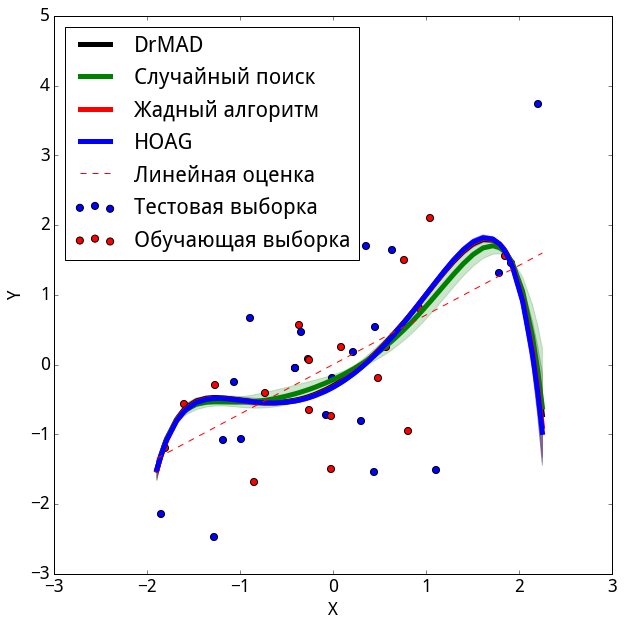
\includegraphics[width=0.8\linewidth]{plots/poly_cv.png}

    \end{subfigure}
    \begin{subfigure}[b]{0.5\textwidth}
    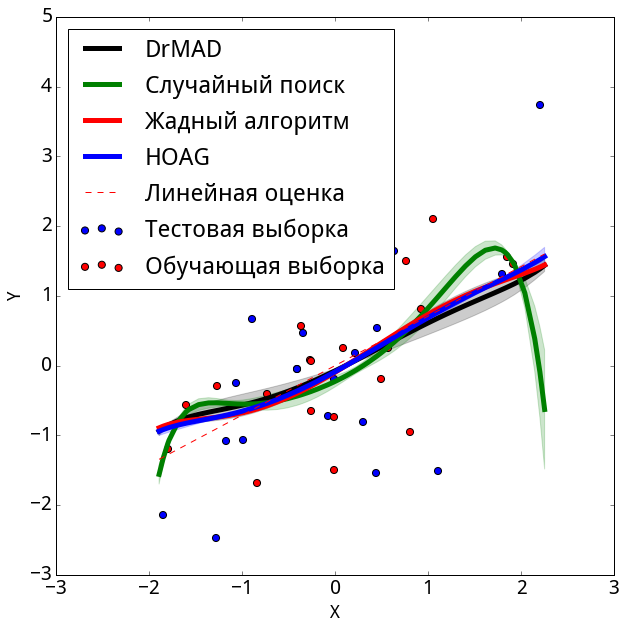
\includegraphics[width=0.8\linewidth]{plots/poly_var.png}

    \end{subfigure}

  \label{fig:poly}
    \caption{Графики итоговых полиномов для синтетической выборки: а --- кросс-валидация, b --- вариационная оценка}
    \end{figure}




    \begin{figure}

    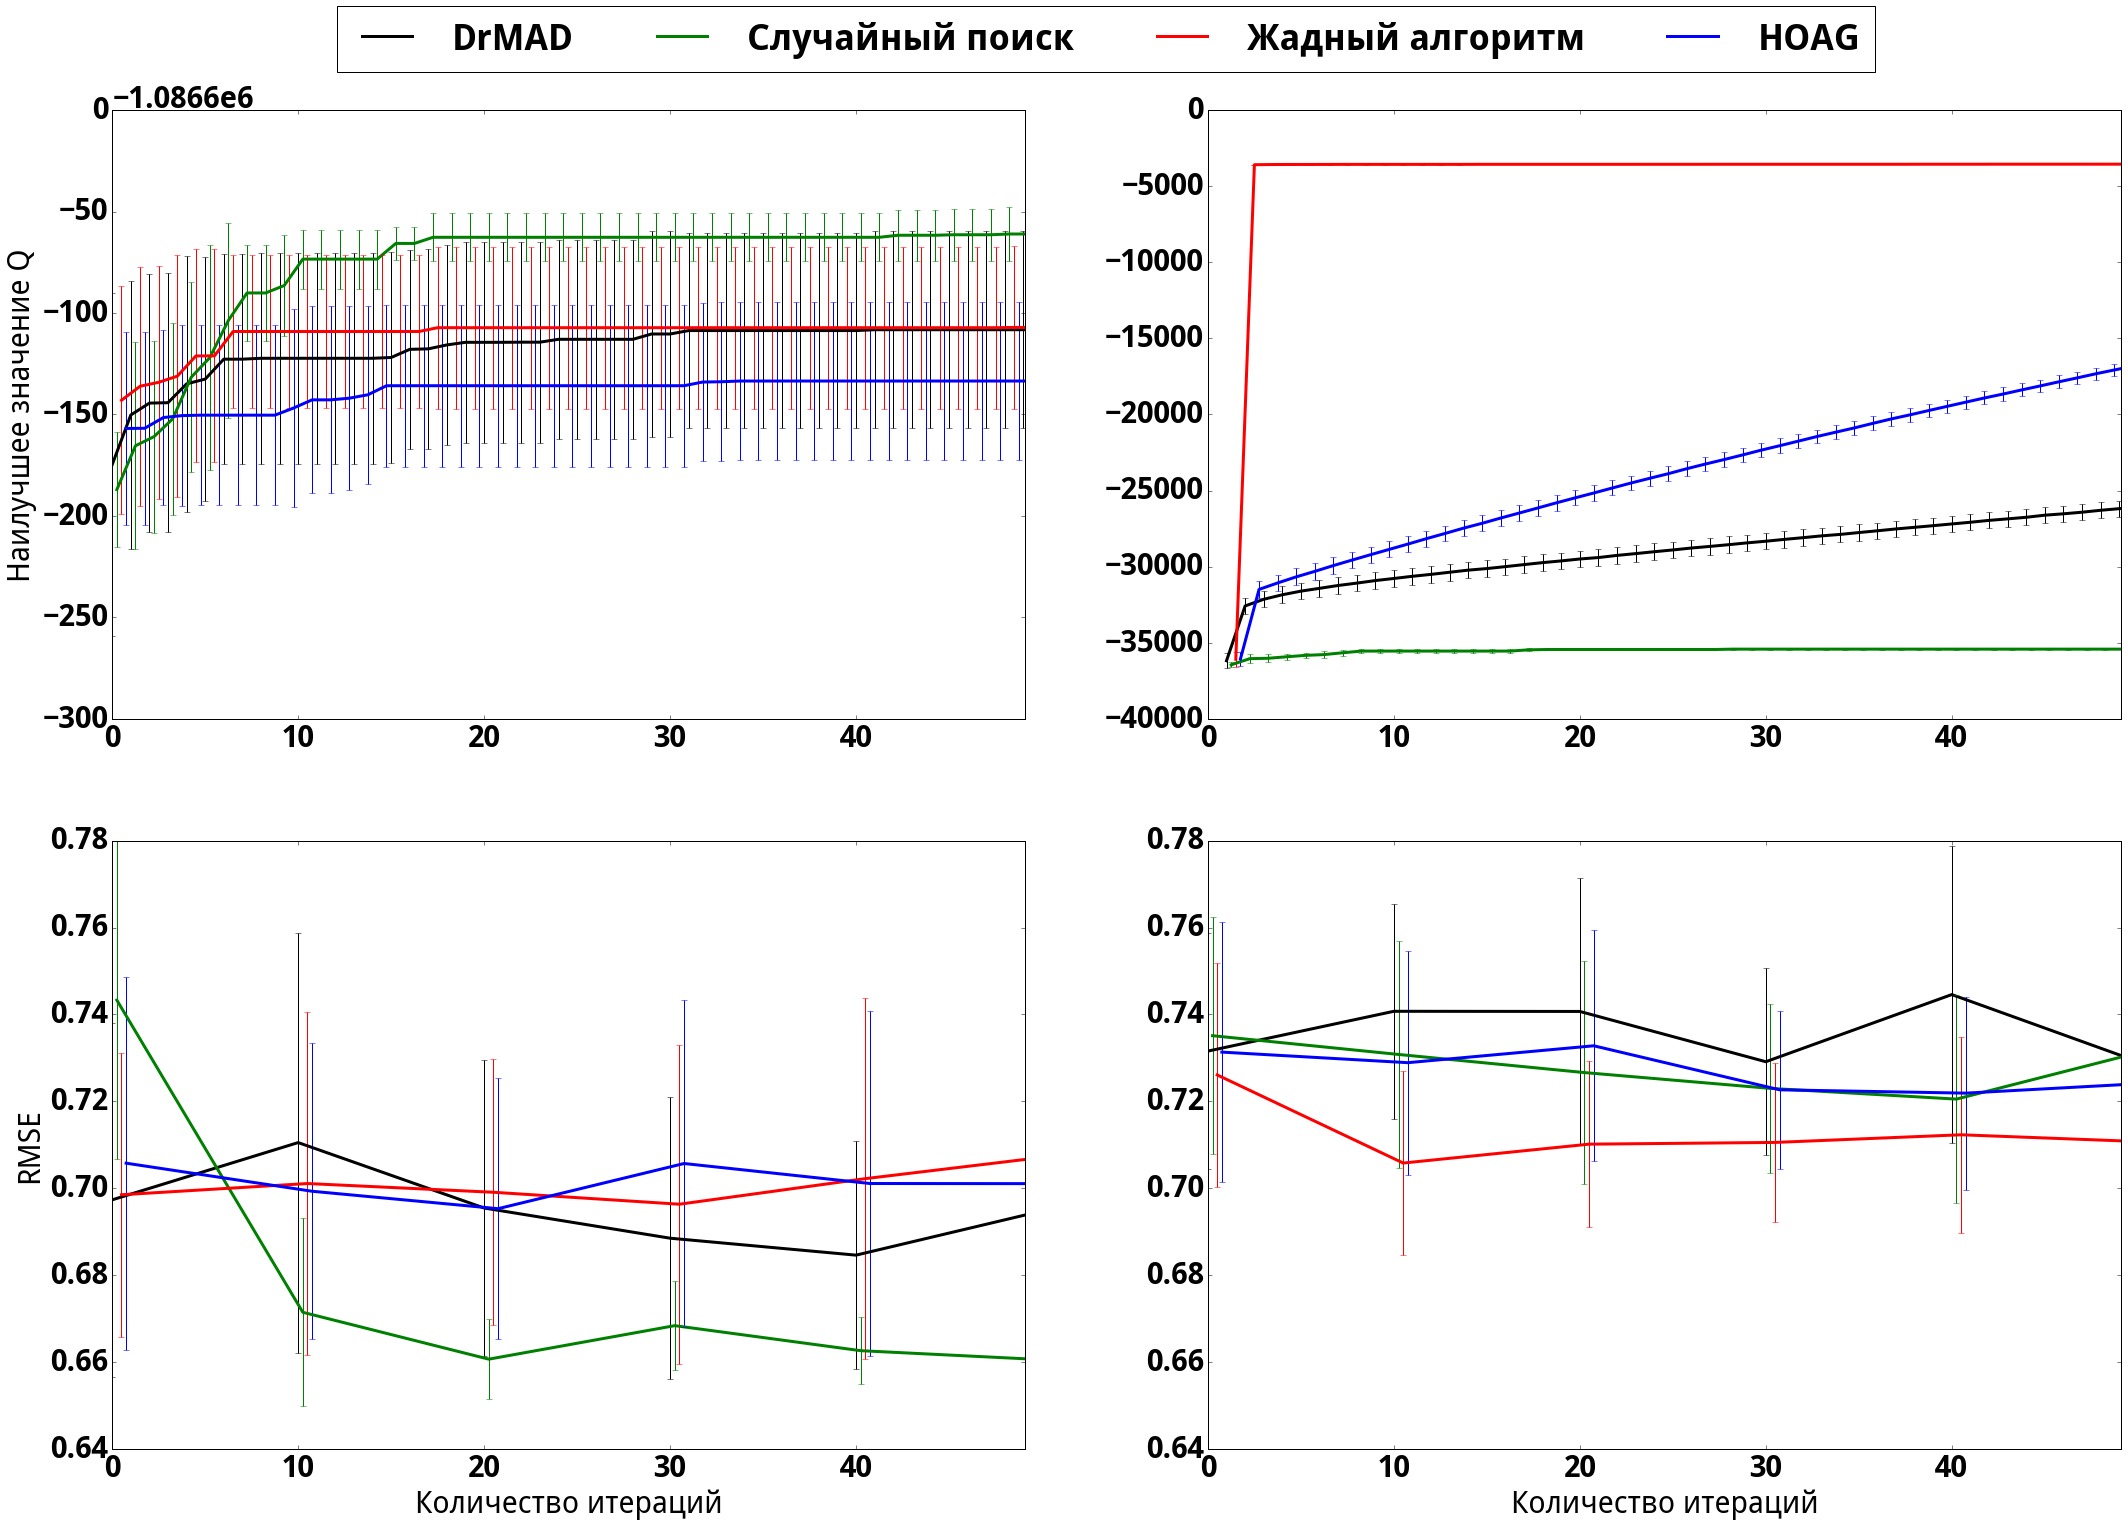
\includegraphics[width=\linewidth]{plots/wisdm.png}

    \caption{Графики завивисимости функции $\hat{Q}$ и качества модели от количества итераций оптимизации для кросс-валидации:  кросс-валидация (слева), вариационная оценка (справа)}
    \end{figure}



\subsection{Модели парафраза (Смердов)}
Цель эксперимента~--- проверка работоспособности предложенного алгоритма и сравнение результатов с ранее полученными. В качестве данных использовалась выборка SemEval 2015, состоящая из 8331 пары схожих и несхожих предложений. Слова преобразовывались в векторы размерности 50 при помощи алгоритма GloVe~\cite{GloveURL}.
%\footnote{https://github.com/stanfordnlp/GloVe}
Для базовых алгоритмов тренировочная, валидационная и тестовая выборки составили 70\%, 15\% и 15\% соответственно.
Для рекуррентной нейронной сети, полученной вариационным методом, валидационная выборка отсутствовала, а тренировочная и тестовая выборки составили 85\% и 15\% соответственно.
Критерием качества была выбрана F1-мера.
В качестве базовых алгоритмов использовались линейная регрессия, метод ближайших соседей, решающее дерево и модификация метода опорных векторов SVC. Базовые алгоритмы взяты из библиотеки sklearn. 
%\cite{sklearn}.
%\footnote{http://scikit-learn.org/stable/}.
Дополнительно были построены рекуррентная нейросеть с одним скрытым слоем~\cite{Sanborn} и нейросеть с одним скрытым слоем и вариационной оптимизацией параметров~\cite{Graves, code}.
% \footnote{https://sourceforge.net/p/mlalgorithms/code/HEAD/tree/Group474/Smerdov2017Paraphrase/code/}.

% Как показал вычислительный эксперимент, вариационная нейросеть, полученная методом, описанным в~\cite{Graves}, позволяет значительно улучшить качество предсказаний.
\begin{figure}[!h]
	\centering
	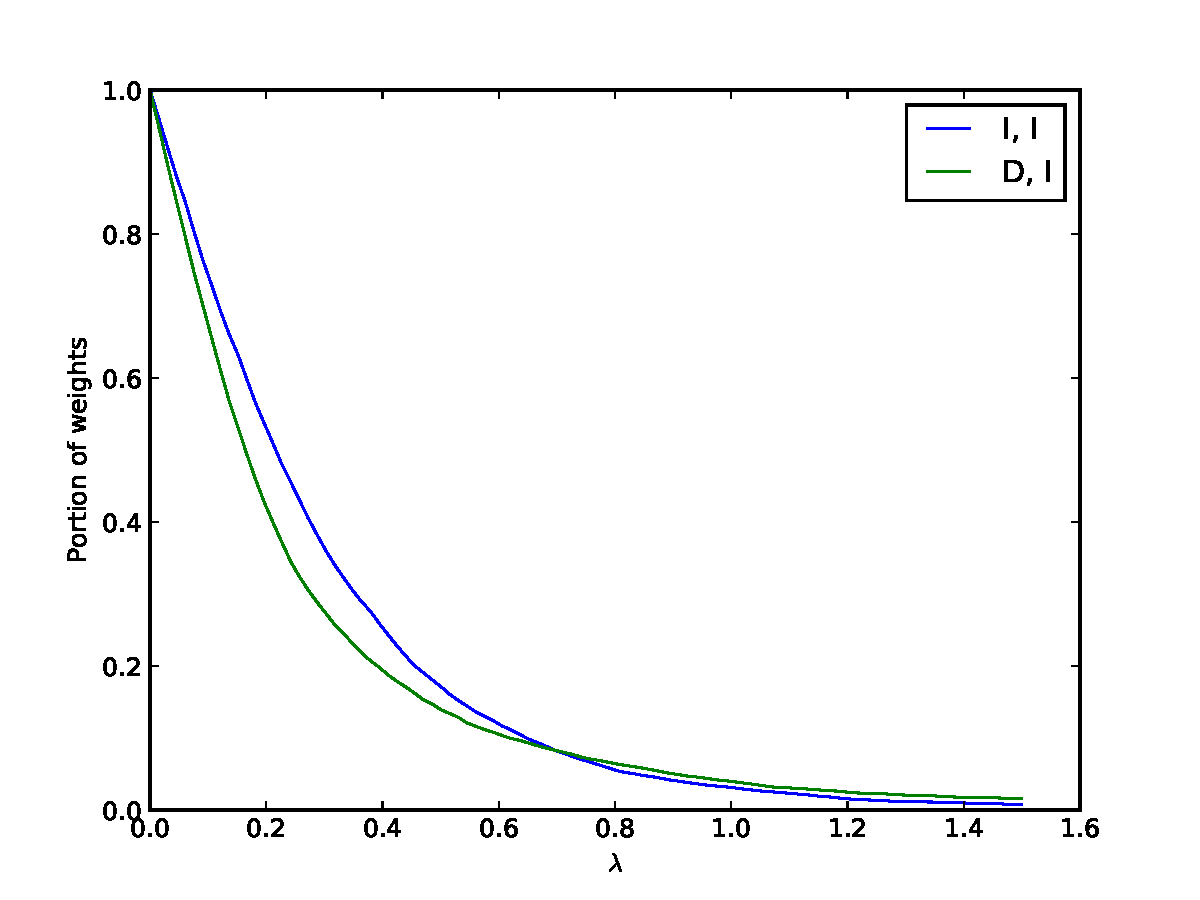
\includegraphics[width=0.5\textwidth]{Pictures/lambdas.pdf}
	\caption{Доля неудаленных параметров сети в зависимости от порогового значения $\lambda$ для скалярного~($I$) и диагонального~($D$) вида апостериорной матрицы ковариаций}
	\label{lambdas}
\end{figure}

 

На рис.~\ref{evidence_I_I} и~\ref{evidence_I_D} представлена зависимость оценки правдоподобия $L$ \eqref{loss} от параметра $\lambda$.
%Видно, что существует некоторое оптимальное значения $\lambda$, при котором оценка минимальна --- именно это значение $\lambda$ соответствует оптимальной модели.
Для обоих случаев существует оптимальное значение $\lambda$, минимизирующее $L$; модели с таким параметром будут оптимальными. На рис.~\ref{score_I_I},~\ref{score_I_D},~\ref{portion_I_I} и~\ref{portion_I_D} отображены зависимости качества модели от $\lambda$ и доли выброшенных параметров. Видно, что даже при удалении большинства параметров из сети качество предсказаний меняется несущественно, что говорит о слишком большом числе параметров исходной модели.

Из рис.~\ref{lambdas} видно, что при малых $\lambda$ из сети с диагональной апостериорной матрицей ковариаций удаляется больше весов, а при больших $\lambda$ --- меньше, что говорит о лучшем отборе параметров такой моделью.


\subsection{Прореживание модели (Грабовой)}
Для анализа свойств предложенного алгоритма и сравнения его с существующими был проведен вычислительный эксперимент в котором параметры нейросети удалялись методами,  которые были описаны в разделах 3.1---3.3 и методом Белсли.

В качестве данных использовались три выборки. Выборки Wine~\cite{Wine} и Boston~Housing~\cite{Boston}  --- это реальные данные. Синтетические данные сгенерированы таким образом чтобы параметры сети были мультиколинеарными. Генерация данных состояла из двух этапов. 
На первом этапе генерировался вектор параметров $\mathbf{w}_{\text{synthetic}}$:
$$\mathbf{w}_{\text{synthetic}}  \sim \mathcal{N}(\textbf{m}_{\text{synthetic}}, \textbf{A}_{\text{synthetic}}), \eqno(5.1)$$ 
где 
$\textbf{m}_{\text{synthetic}} = \begin{bmatrix}
1.0\\
0.0025\\
\cdots\\
0.0025
\end{bmatrix}$,
$\textbf{A}_{\text{synthetic}} = \begin{bmatrix}
1.0& 10^{-3}& \cdots& 10^{-3}& 10^{-3}\\
10^{-3}& 1.0& \cdots& 0.95& 0.95\\
\cdots&\cdots&\cdots&\cdots&\cdots\\
10^{-3}& 0.95& \cdots& 0.95& 1.0
\end{bmatrix}$.

На втором этапе генерировалась выборка $\mathfrak{D}_{\text{synthetic}}$:
$$\mathfrak{D}_{\text{synthetic}} = \{(\textbf{x}_i,y_i)| \textbf{x}_i \sim  \mathcal{N}(\textbf{1}, \textbf{I}), y_i = x_{i0}, i = 1 \cdots 10000\}. \eqno(5.2)$$
В приведенном выше векторе параметров $\mathbf{w}_{\text{synthetic}}$ для выборки $\mathfrak{D}_{\text{synthetic}}$, наиболее релевантным является первый параметр, а все остальные параметры являются нерелевантными. Матрица ковариации была выбрана таким образом, чтобы все нерелевантные параметры были зависимы и метод Белсли был максимально эффективен.



\begin{table}[h]

\begin{center}
\caption{Описание выборок}
\begin{tabular}{|c|c|c|c|}
\hline
	Выборка &Тип задачи& Размер выборки& Число признаков\\
	\hline
	
	\multicolumn{1}{|l|}{Wine}
	&
	\multicolumn{1}{|l|}{класификация}
	 & 178 & 13\\
	\hline
	
	\multicolumn{1}{|l|}{Boston Housing}
	&
	\multicolumn{1}{|l|}{регресия}
	& 506 & 13\\
	\hline
	
	\multicolumn{1}{|l|}{Synthetic data}
	&
	\multicolumn{1}{|l|}{регресия}
	& 10000 & 100\\
\hline

\end{tabular}
\end{center}
\end{table}



Для алгоритмов тренировочная и тестовая выборки составили~$80\%$ и~$20\%$ соответсвенно. Критерием качества прореживания служит процент параметров нейросети, удаление которого не влечет значимой потери качества прогноза. Также критерием качества служит устойчивость нейросети к зашумленности данных. 

Качеством прогноза $R_{\text{cl}}$ модели для задачи классификации является точность прогноза модели:
$$R_{\text{cl}} = \frac{\sum_{(\textbf{x},y)\in \mathfrak{D}} [f(\textbf{x}, \textbf{w}) = y]}{\left|\mathfrak{D}\right|}, \eqno(5.3)$$

Качеством прогноза $R_{\text{rg}} $ модели для задачи регрессии является среднеквадратическое отклонение результата модели от точного:

$$R_{\text{rg}} = \frac{\sum_{(\textbf{x},y)\in \mathfrak{D}} \left(f(\textbf{x}, \textbf{w}) - y\right)^2}{\left|\mathfrak{D}\right|}, \eqno(5.4)$$

\textbf{Wine.} Рассмотрим нейроную сеть с 13 нейронами на входе, 13 нейронами в скрытом слое и 3 нейронами на выходе.

\begin{figure}[h!t]\center
\includegraphics[width=0.8\textwidth]{results/New/WIne/All.pdf}\\
\caption{Качество прогноза при удаление параметров на выборке Wine}
\label{WineAll}
\end{figure}

\begin{figure}[h!t]\center
\subfloat[Произвольное удаление параметров]{\includegraphics[width=0.5\textwidth]{results/New/WIne/RandomNoise3D.pdf}}
\subfloat[Оптимальное прореживание]{\includegraphics[width=0.5\textwidth]{results/New/WIne/OBDNoise3D.pdf}}\\
\subfloat[Вариационный метод]{\includegraphics[width=0.5\textwidth]{results/New/WIne/VariationalNoise3D.pdf}}
\caption{Влияние шума в начальных данных на шум выхода нейросети на выборке Wine}
\label{WineNoise}
\end{figure}

На рис.~\ref{WineAll} показано как меняется точность прогноза $R_{\text{cl}}$ при удалении параметров указанными методами. Из графика видно, что метод оптимального прореживания, вариационный метод и метод Белсли позволяют удалить $\approx80\%$ параметров и качество всех этих методов падает при удалении $\approx90\%$ параметров нейросети. 

На рис.~\ref{WineNoise} показаны поверхности изменения уровня шума ответов нейросети при изменении процента удаленных параметров и уровня шума входных данных для разных методов прореживания. На графиках показано, что при удалении параметров нейросети методом Белсли шум меньше, чем при удалении параметров другими методами, на это указывает то что поверхность которая соответствует методу Белсли ниже других поверхностей.

\textbf{Boston Housing. } Рассмотрим нейроную сеть с 13 нейронами на входе, 39 нейронами в скрытом слое и одним нейроном на выходе.

\begin{figure}[h!t]\center
\includegraphics[width=0.8\textwidth]{results/New/Boston/All.pdf}\\
\caption{Качество прогноза при удаление параметров на выборке Boston}
\label{BostonAll}
\end{figure}

\begin{figure}[h!t]\center
\subfloat[Произвольное удаление параметров]{\includegraphics[width=0.5\textwidth]{results/New/Boston/RandomNoise3D.pdf}}
\subfloat[Оптимальное прореживание]{\includegraphics[width=0.5\textwidth]{results/New/Boston/OBDNoise3D.pdf}}\\
\subfloat[Вариационный метод]{\includegraphics[width=0.5\textwidth]{results/New/Boston/VariationalNoise3D.pdf}}
\caption{Влияние шума в начальных данных на шум выхода нейросети на выборке Boston}
\label{BostonNoise}
\end{figure}

На рис.~\ref{BostonAll} показано как меняется среднеквадратическое отклонение прогноза $\mathsf{R}_{\text{rg}}$ от точного ответа  при удалении параметров указанными методами. График показывает, что метод Белсли является более эффективным, чем другие методы, так-как позволяет удалить больше параметров нейросети без потери качества.

На рис.~\ref{BostonNoise} показаны поверхности изменения уровня шума ответов нейросети при изменении процента удаленных параметров и уровня шума входных данных для разных методов прореживания. График показывает, что уровень шума всех методов одинаковый, так-как поверхности всех методов находятся на одном уровне.


\textbf{Синтетические данные. } Рассмотрим нейроную сеть с 100 нейронами на входе и одним нейроном на выходе.

\begin{figure}[h!t]\center
\includegraphics[width=0.8\textwidth]{results/New/Data1/All.pdf}\\
\caption{Качество прогноза при удаление параметров на синтетической выборке}
\label{Data1All}
\end{figure}

\begin{figure}[h!t]\center
\subfloat[Произвольное удаление параметров]{\includegraphics[width=0.5\textwidth]{results/New/Data1/RandomNoise3D.pdf}}
\subfloat[Оптимальное прореживание]{\includegraphics[width=0.5\textwidth]{results/New/Data1/OBDNoise3D.pdf}}\\
\subfloat[Вариационный метод]{\includegraphics[width=0.5\textwidth]{results/New/Data1/VariationalNoise3D.pdf}}
\caption{Влияние шума в начальных данных на шум выхода нейросети на синтетической выборке}
\label{Data1Noise}
\end{figure}

На рис.~\ref{Data1All} показано как меняется среднеквадратическое отклонение прогноза от $\mathsf{R}_{\text{rg}}$ точного ответа при удалении параметров указанными методами. График показывает, что удаление параметров методом Белсли являеться более эффективным чем другие методы прореживания, так-как качество прогноза нейросети улучшается при удалении шумовых параметров.

На рис.~\ref{Data1Noise} показаны поверхности изменения уровня шума ответов нейросети при изменении процента удаленных параметров и уровня шума входных данных для разных методов прореживания. На графиках показано, что при удалении параметров нейросети методом Белсли шум меньше, чем при удалении параметров другими методами, так-как поверхность которая соответствует методу Белсли ниже других поверхностей.



